% Présentation de TeX et LaTeX
\small

\section{\TeX\ and \LaTeX\ presentation}

\subsection{What is \TeX\ and \LaTeX?}

\begin{frame}[c,label=fr:commencement]{At the beginning (1978), there was \TeX\ldots}
	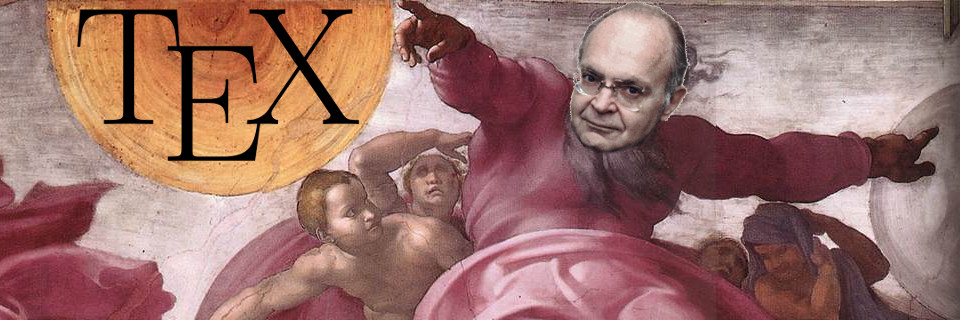
\includegraphics[width=\textwidth,keepaspectratio=true]{knuth-tex-commencement.jpg}
\end{frame}

\begin{frame}[c]{What is \TeX?}

	\begin{itemize}
		\item A typesetting and document preparation system;
		\item ``The most powerful formatting program for producing book-quality text 
			of scientific and technical works''\footnote{Kopka \& Daly, p. 6};
		\item A mature, stable, complete and bug-free system;
		\item A set of very primitive commands perfect for typography and
			programming functions;
		\item «\emph{typesetter-level program}».
	\end{itemize}

\end{frame}

\begin{frame}[c,label=fr:sixiemejour]{On the sixth day (1983), there was \LaTeX\ldots}
	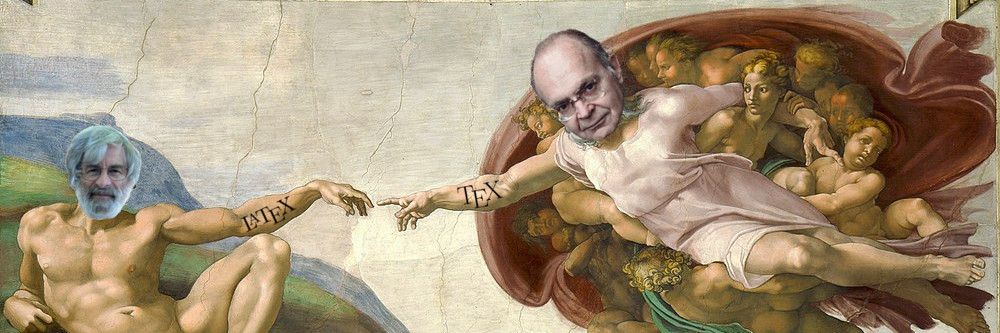
\includegraphics[width=\textwidth,keepaspectratio=true]{creation-of-latex.jpg}
\end{frame}

\begin{frame}{What is \LaTeX?}
	\begin{itemize}
		\item A set of macro-commands used to facilitate \TeX's usage;
		\item No preliminary knowledge of typography in general or \TeX\ in particular
			is required;
		\item Typographical and logical markup language used for text layout (like HTML);
		\item Cross-platform language, identical from one operating system to the other,
			and extensible with packages;
		\item «\emph{author-level program}».
	\end{itemize}
\end{frame}

\subsection{A \LaTeX\ document creation process}

% Rédiger avec une nouvelle perspective
\begin{frame}[c]{Writing with a new perspective}
	
	\begin{itemize}
		\item You write your document in plain text and use commands to describe
			\textbf{what your text is} and \textbf{not what it's supposed to look like}.
		\item You concentrate on your \textbf{content}.
		\item You let \LaTeX\ do its work, that is taking care of the \textbf{container}.
	\end{itemize}
	
\end{frame}

% Processus de création d'un document LaTeX
\begin{frame}[c]{\LaTeX\ document creation process}
	\Huge
	\begin{minipage}[t]{0.25\linewidth}
		\centering
		\faFileTextO
	\end{minipage}
	\hfill\faArrowRight\hfill
	\begin{minipage}[t]{0.25\linewidth}
		\centering
		\faCogs
	\end{minipage}
	\hfill\faArrowRight\hfill
	\begin{minipage}[t]{0.25\linewidth}
		\centering
		\faFilePdfO
	\end{minipage}

	\begin{picture}(0,0)
		\footnotesize\thicklines\color{bleuFonceSecondaire}
		\onslide<2>\put(0,-10){\dashbox{1}(35,40)[b]{\parbox{.2\textwidth}{\centering\textbf{text writing and markup in a text editor\smallskip}}}}
		\onslide<3>\put(54,-10){\dashbox{1}(35,40)[b]{\parbox{.2\textwidth}{\centering\textbf{compilation with a \TeX\ engine from the command line\smallskip}}}}
		\onslide<4>\put(108,-10){\dashbox{1}(35,40)[b]{\parbox{.2\textwidth}{\centering\textbf{visualization with an external viewer\smallskip}}}}
	\end{picture}
\end{frame}